\chapter{CPVC 润滑剂对 CPVC 热稳定性和力学性能作用研究}

\section{配方设计}
本实验中使用了 1 种聚乙烯蜡:PEW-0380 以及 3 种氧化聚乙烯蜡:AC-316、AC-617、AC-629。聚乙烯蜡为乙烯的低度聚合产品,具有良好的中期及后期润滑性,并能在 CPVC 注塑加工中作为脱模剂使用。氧化聚乙烯蜡为含羧基的低分子量聚乙烯,并含有醇、酮及酯类化合物。由于氧化使烷烃链上生成一定数量极性的羧基,提高了它在 CPVC 的相容性,使其同时兼有良好的内、外润滑性能,并赋予制品良好的透明性和光泽性。\par
在这一部分实验中,主要比较这 4 种外润滑剂对于 CPVC 热稳定性和力学性能的影响。通过保持其他助剂的种类和含量不变,独立改变外润滑剂的种类设计了 4 种配方,具体配方如表 \ref{tabSmoothPre} 所示。

\begin{table}[!htbp]
    \caption{CPVC 4 种外润滑剂配方设计表}
    \label{tabSmoothPre}
    \begin{center}
    \footnotesize{
        \begin{tabular}{ccccccccccc}
            \Xhline{1pt}
            组别 & CPVC & \makecell[c]{抗冲击\\改性剂} & 有机锡 & \makecell[c]{AC-\\316} & \makecell[c]{AC-\\617} & \makecell[c]{AC-\\629} & \makecell[c]{PEW-\\0380} & \makecell[c]{汉高\\G-60} & \makecell[c]{加工\\助剂} & \makecell[c]{钛白粉}   \\
            \Xhline{0.5pt}
            $E_1$ & 100 & 8 & 2 & 1.3 & & & & 1.2 & 3 & 2   \\
            $E_2$ & 100 & 8 & 2 & & 1.3 & & & 1.2 & 3 & 2   \\
            $E_3$ & 100 & 8 & 2 & & & 1.3 & & 1.2 & 3 & 2   \\
            $E_4$ & 100 & 8 & 2 & & & & 1.3 & 1.2 & 3 & 2   \\
            \Xhline{1pt}
        \end{tabular}
    }
    \end{center}
\end{table}


\section{外润滑剂种类对 CPVC 动态热稳定性的影响}

图 \ref{fig1Hakee} 所示为 E1$\sim$E4 4 种配方在转矩流变仪中进行加热剪切过程的 转矩-时间 曲线。

\begin{figure}[!htbp]
    \begin{center}
        % GNUPLOT: LaTeX picture with Postscript
\begingroup
  \makeatletter
  \providecommand\color[2][]{%
    \GenericError{(gnuplot) \space\space\space\@spaces}{%
      Package color not loaded in conjunction with
      terminal option `colourtext'%
    }{See the gnuplot documentation for explanation.%
    }{Either use 'blacktext' in gnuplot or load the package
      color.sty in LaTeX.}%
    \renewcommand\color[2][]{}%
  }%
  \providecommand\includegraphics[2][]{%
    \GenericError{(gnuplot) \space\space\space\@spaces}{%
      Package graphicx or graphics not loaded%
    }{See the gnuplot documentation for explanation.%
    }{The gnuplot epslatex terminal needs graphicx.sty or graphics.sty.}%
    \renewcommand\includegraphics[2][]{}%
  }%
  \providecommand\rotatebox[2]{#2}%
  \@ifundefined{ifGPcolor}{%
    \newif\ifGPcolor
    \GPcolorfalse
  }{}%
  \@ifundefined{ifGPblacktext}{%
    \newif\ifGPblacktext
    \GPblacktexttrue
  }{}%
  % define a \g@addto@macro without @ in the name:
  \let\gplgaddtomacro\g@addto@macro
  % define empty templates for all commands taking text:
  \gdef\gplbacktext{}%
  \gdef\gplfronttext{}%
  \makeatother
  \ifGPblacktext
    % no textcolor at all
    \def\colorrgb#1{}%
    \def\colorgray#1{}%
  \else
    % gray or color?
    \ifGPcolor
      \def\colorrgb#1{\color[rgb]{#1}}%
      \def\colorgray#1{\color[gray]{#1}}%
      \expandafter\def\csname LTw\endcsname{\color{white}}%
      \expandafter\def\csname LTb\endcsname{\color{black}}%
      \expandafter\def\csname LTa\endcsname{\color{black}}%
      \expandafter\def\csname LT0\endcsname{\color[rgb]{1,0,0}}%
      \expandafter\def\csname LT1\endcsname{\color[rgb]{0,1,0}}%
      \expandafter\def\csname LT2\endcsname{\color[rgb]{0,0,1}}%
      \expandafter\def\csname LT3\endcsname{\color[rgb]{1,0,1}}%
      \expandafter\def\csname LT4\endcsname{\color[rgb]{0,1,1}}%
      \expandafter\def\csname LT5\endcsname{\color[rgb]{1,1,0}}%
      \expandafter\def\csname LT6\endcsname{\color[rgb]{0,0,0}}%
      \expandafter\def\csname LT7\endcsname{\color[rgb]{1,0.3,0}}%
      \expandafter\def\csname LT8\endcsname{\color[rgb]{0.5,0.5,0.5}}%
    \else
      % gray
      \def\colorrgb#1{\color{black}}%
      \def\colorgray#1{\color[gray]{#1}}%
      \expandafter\def\csname LTw\endcsname{\color{white}}%
      \expandafter\def\csname LTb\endcsname{\color{black}}%
      \expandafter\def\csname LTa\endcsname{\color{black}}%
      \expandafter\def\csname LT0\endcsname{\color{black}}%
      \expandafter\def\csname LT1\endcsname{\color{black}}%
      \expandafter\def\csname LT2\endcsname{\color{black}}%
      \expandafter\def\csname LT3\endcsname{\color{black}}%
      \expandafter\def\csname LT4\endcsname{\color{black}}%
      \expandafter\def\csname LT5\endcsname{\color{black}}%
      \expandafter\def\csname LT6\endcsname{\color{black}}%
      \expandafter\def\csname LT7\endcsname{\color{black}}%
      \expandafter\def\csname LT8\endcsname{\color{black}}%
    \fi
  \fi
    \setlength{\unitlength}{0.0500bp}%
    \ifx\gptboxheight\undefined%
      \newlength{\gptboxheight}%
      \newlength{\gptboxwidth}%
      \newsavebox{\gptboxtext}%
    \fi%
    \setlength{\fboxrule}{0.5pt}%
    \setlength{\fboxsep}{1pt}%
\begin{picture}(7200.00,5040.00)%
    \gplgaddtomacro\gplbacktext{%
      \csname LTb\endcsname%
      \put(814,704){\makebox(0,0)[r]{\strut{}$-10$}}%
      \put(814,1213){\makebox(0,0)[r]{\strut{}$-5$}}%
      \put(814,1722){\makebox(0,0)[r]{\strut{}$0$}}%
      \put(814,2231){\makebox(0,0)[r]{\strut{}$5$}}%
      \put(814,2740){\makebox(0,0)[r]{\strut{}$10$}}%
      \put(814,3248){\makebox(0,0)[r]{\strut{}$15$}}%
      \put(814,3757){\makebox(0,0)[r]{\strut{}$20$}}%
      \put(814,4266){\makebox(0,0)[r]{\strut{}$25$}}%
      \put(814,4775){\makebox(0,0)[r]{\strut{}$30$}}%
      \put(946,484){\makebox(0,0){\strut{}$0$}}%
      \put(1678,484){\makebox(0,0){\strut{}$1$}}%
      \put(2410,484){\makebox(0,0){\strut{}$2$}}%
      \put(3142,484){\makebox(0,0){\strut{}$3$}}%
      \put(3875,484){\makebox(0,0){\strut{}$4$}}%
      \put(4607,484){\makebox(0,0){\strut{}$5$}}%
      \put(5339,484){\makebox(0,0){\strut{}$6$}}%
      \put(6071,484){\makebox(0,0){\strut{}$7$}}%
      \put(6803,484){\makebox(0,0){\strut{}$8$}}%
    }%
    \gplgaddtomacro\gplfronttext{%
      \csname LTb\endcsname%
      \put(176,2739){\rotatebox{-270}{\makebox(0,0){\strut{}转矩/N$\cdot$m}}}%
      \put(3874,154){\makebox(0,0){\strut{}时间/min}}%
      \csname LTb\endcsname%
      \put(5816,1537){\makebox(0,0)[r]{\strut{}AC-316}}%
      \csname LTb\endcsname%
      \put(5816,1317){\makebox(0,0)[r]{\strut{}AC-617}}%
      \csname LTb\endcsname%
      \put(5816,1097){\makebox(0,0)[r]{\strut{}AC-629}}%
      \csname LTb\endcsname%
      \put(5816,877){\makebox(0,0)[r]{\strut{}PEW-0380}}%
    }%
    \gplbacktext
    \put(0,0){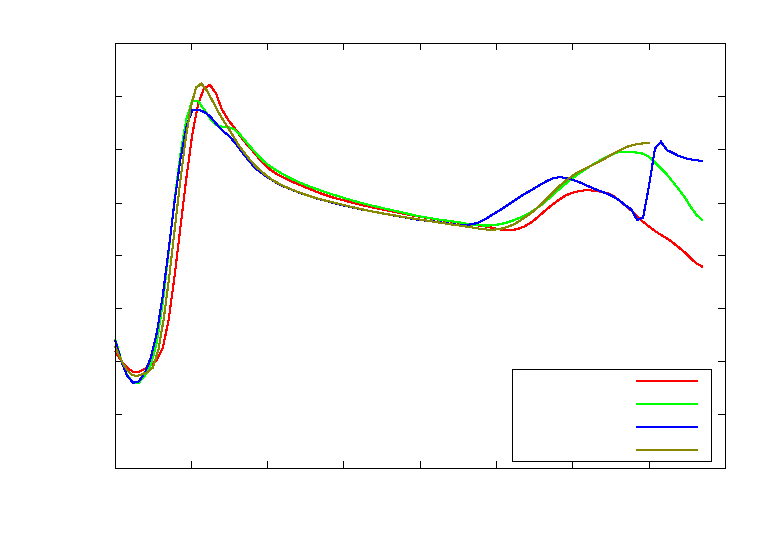
\includegraphics{src/origin/1/hakee}}%
    \gplfronttext
  \end{picture}%
\endgroup

    \end{center}
    \caption{外润滑剂动态热稳定性}
    \label{fig1Hakee}
\end{figure}

由图 \ref{fig1Hakee} 可得到该体系的熔化转矩、平衡转矩与热稳定时间\footnote{见 \pageref{sectionHakee} 页 \ref{sectionHakee} 动态热稳定性},具体数据见表 \ref{tab1Hakee}所示。

\begin{table}[!htbp]
    \caption{动态热稳定性能数据表}
    \label{tab1Hakee}
    \begin{center}
    \footnotesize{
        \begin{tabular}{ccccc}
            \Xhline{1pt}
            组别 & 润滑剂种类 & \makecell[c]{熔化转矩 $M_{fus}$/\\N$\cdot$m} & \makecell[c]{平衡转矩$M_{melt}$/\\N$\cdot$m} & \makecell[c]{热稳定时间$T_{s}$/\\min} \\
            \Xhline{0.5pt}
            $E_1$ & AC-316 & 29.6 & 12.1 & 6.2  \\
            $E_2$ & AC-617 & 26.5 & 12.5 & 6.6  \\
            $E_3$ & AC-629 & 24.9 & 12.4 & 5.9  \\
            $E_4$ & PEW-0380 & 28.0 & 12.2 & 7.3    \\
            \Xhline{1pt}
        \end{tabular}
    }
    \end{center}
\end{table}

结合图表数据可以看出,$E_3$ 组配方具有最小的熔化转矩,为 24.9 N$\cdot$m,剩余组别顺序依次为 $M_{fus, E_2}$ < $M_{fus, E_4}$ < $M_{fus, E_1}$。4 组的平衡转矩相差不大,顺序依次为 $M_{melt, E_1}$ < $M_{melt, E_4}$ < $M_{melt, E_3}$ < $M_{melt, E_2}$,AC-316 与 PEW-0380 对于 CPVC 加工性能的改善略优于 AC-617 与 AC-629。$E_4$ 组的 $T_{s}$ 为 7.3 min,能够满足 CPVC 塑化加工的要求。

\section{静态热稳定性}

\begin{table}[!htbp]
    \caption{热烘箱法测定样品颜色随时间变化}
    \label{tab1static}
    \begin{center}
    \footnotesize{
        \begin{tabular}{cccccccc}
            \Xhline{1pt}
            \multirow{2}{*}{Sample} & \multicolumn{7}{c}{加入不同种类稳定剂的 CPVC 试样 180\cd 烘箱中颜色随时间的变化}\\
            \cline{2-8}
            & 0 min & 20 min & 30 min & 70 min & 120 min & 250 min & 360 min  \\
            \Xhline{0.5pt} 
            $E_1$ & \makecell[c]{
\includegraphics[width=.1\linewidth]{src/origin/1/static/00.png}} & \makecell[c]{
\includegraphics[width=.1\linewidth]{src/origin/1/static/01.png}} & \makecell[c]{
\includegraphics[width=.1\linewidth]{src/origin/1/static/02.png}} & \makecell[c]{
\includegraphics[width=.1\linewidth]{src/origin/1/static/03.png}} & \makecell[c]{
\includegraphics[width=.1\linewidth]{src/origin/1/static/04.png}} & \makecell[c]{
\includegraphics[width=.1\linewidth]{src/origin/1/static/05.png}} & \makecell[c]{
\includegraphics[width=.1\linewidth]{src/origin/1/static/06.png}}   \\
            $E_2$ & \makecell[c]{
\includegraphics[width=.1\linewidth]{src/origin/1/static/10.png}} & \makecell[c]{
\includegraphics[width=.1\linewidth]{src/origin/1/static/11.png}} & \makecell[c]{
\includegraphics[width=.1\linewidth]{src/origin/1/static/12.png}} & \makecell[c]{
\includegraphics[width=.1\linewidth]{src/origin/1/static/13.png}} & \makecell[c]{
\includegraphics[width=.1\linewidth]{src/origin/1/static/14.png}} & \makecell[c]{
\includegraphics[width=.1\linewidth]{src/origin/1/static/15.png}} & \makecell[c]{
\includegraphics[width=.1\linewidth]{src/origin/1/static/16.png}}  \\
            $E_3$ & \makecell[c]{
\includegraphics[width=.1\linewidth]{src/origin/1/static/20.png}} & \makecell[c]{
\includegraphics[width=.1\linewidth]{src/origin/1/static/21.png}} & \makecell[c]{
\includegraphics[width=.1\linewidth]{src/origin/1/static/22.png}} & \makecell[c]{
\includegraphics[width=.1\linewidth]{src/origin/1/static/23.png}} & \makecell[c]{
\includegraphics[width=.1\linewidth]{src/origin/1/static/24.png}} & \makecell[c]{
\includegraphics[width=.1\linewidth]{src/origin/1/static/25.png}} & \makecell[c]{
\includegraphics[width=.1\linewidth]{src/origin/1/static/26.png}}  \\
            $E_4$ & \makecell[c]{
\includegraphics[width=.1\linewidth]{src/origin/1/static/30.png}} & \makecell[c]{
\includegraphics[width=.1\linewidth]{src/origin/1/static/31.png}} & \makecell[c]{
\includegraphics[width=.1\linewidth]{src/origin/1/static/32.png}} & \makecell[c]{
\includegraphics[width=.1\linewidth]{src/origin/1/static/33.png}} & \makecell[c]{
\includegraphics[width=.1\linewidth]{src/origin/1/static/34.png}} & \makecell[c]{
\includegraphics[width=.1\linewidth]{src/origin/1/static/35.png}} & \makecell[c]{
\includegraphics[width=.1\linewidth]{src/origin/1/static/36.png}}    \\
            \Xhline{1pt}
        \end{tabular}
    }
    \end{center}
\end{table}

将 4 组配方的样板进行切割,取 1 $\rm{mm^2}$ 的试样进行测试,结果如表 \ref{tab1static} 所示。$E_1$ 组和 $E_2$ 组的样品在实验开始的 20 min 后表面开始出现起伏,当达到 360 min 时,表面已严重变黑且因 CPVC 分解产生 HCl 而形成了大量的气泡。分析原因是 AC-316 与 AC-617 对 CPVC 树脂的塑化改善不大,CPVC 树脂由于塑化不佳致其容易发生分解。$E_4$ 组在 360 min 时轻微发黄,认为 PEW-0380 对 CPVC 塑化效果改善最大。

\section{玻璃化转变温度}

\begin{figure}[!htbp]
    \begin{center}
        % GNUPLOT: LaTeX picture with Postscript
\begingroup
  \makeatletter
  \providecommand\color[2][]{%
    \GenericError{(gnuplot) \space\space\space\@spaces}{%
      Package color not loaded in conjunction with
      terminal option `colourtext'%
    }{See the gnuplot documentation for explanation.%
    }{Either use 'blacktext' in gnuplot or load the package
      color.sty in LaTeX.}%
    \renewcommand\color[2][]{}%
  }%
  \providecommand\includegraphics[2][]{%
    \GenericError{(gnuplot) \space\space\space\@spaces}{%
      Package graphicx or graphics not loaded%
    }{See the gnuplot documentation for explanation.%
    }{The gnuplot epslatex terminal needs graphicx.sty or graphics.sty.}%
    \renewcommand\includegraphics[2][]{}%
  }%
  \providecommand\rotatebox[2]{#2}%
  \@ifundefined{ifGPcolor}{%
    \newif\ifGPcolor
    \GPcolorfalse
  }{}%
  \@ifundefined{ifGPblacktext}{%
    \newif\ifGPblacktext
    \GPblacktexttrue
  }{}%
  % define a \g@addto@macro without @ in the name:
  \let\gplgaddtomacro\g@addto@macro
  % define empty templates for all commands taking text:
  \gdef\gplbacktext{}%
  \gdef\gplfronttext{}%
  \makeatother
  \ifGPblacktext
    % no textcolor at all
    \def\colorrgb#1{}%
    \def\colorgray#1{}%
  \else
    % gray or color?
    \ifGPcolor
      \def\colorrgb#1{\color[rgb]{#1}}%
      \def\colorgray#1{\color[gray]{#1}}%
      \expandafter\def\csname LTw\endcsname{\color{white}}%
      \expandafter\def\csname LTb\endcsname{\color{black}}%
      \expandafter\def\csname LTa\endcsname{\color{black}}%
      \expandafter\def\csname LT0\endcsname{\color[rgb]{1,0,0}}%
      \expandafter\def\csname LT1\endcsname{\color[rgb]{0,1,0}}%
      \expandafter\def\csname LT2\endcsname{\color[rgb]{0,0,1}}%
      \expandafter\def\csname LT3\endcsname{\color[rgb]{1,0,1}}%
      \expandafter\def\csname LT4\endcsname{\color[rgb]{0,1,1}}%
      \expandafter\def\csname LT5\endcsname{\color[rgb]{1,1,0}}%
      \expandafter\def\csname LT6\endcsname{\color[rgb]{0,0,0}}%
      \expandafter\def\csname LT7\endcsname{\color[rgb]{1,0.3,0}}%
      \expandafter\def\csname LT8\endcsname{\color[rgb]{0.5,0.5,0.5}}%
    \else
      % gray
      \def\colorrgb#1{\color{black}}%
      \def\colorgray#1{\color[gray]{#1}}%
      \expandafter\def\csname LTw\endcsname{\color{white}}%
      \expandafter\def\csname LTb\endcsname{\color{black}}%
      \expandafter\def\csname LTa\endcsname{\color{black}}%
      \expandafter\def\csname LT0\endcsname{\color{black}}%
      \expandafter\def\csname LT1\endcsname{\color{black}}%
      \expandafter\def\csname LT2\endcsname{\color{black}}%
      \expandafter\def\csname LT3\endcsname{\color{black}}%
      \expandafter\def\csname LT4\endcsname{\color{black}}%
      \expandafter\def\csname LT5\endcsname{\color{black}}%
      \expandafter\def\csname LT6\endcsname{\color{black}}%
      \expandafter\def\csname LT7\endcsname{\color{black}}%
      \expandafter\def\csname LT8\endcsname{\color{black}}%
    \fi
  \fi
    \setlength{\unitlength}{0.0500bp}%
    \ifx\gptboxheight\undefined%
      \newlength{\gptboxheight}%
      \newlength{\gptboxwidth}%
      \newsavebox{\gptboxtext}%
    \fi%
    \setlength{\fboxrule}{0.5pt}%
    \setlength{\fboxsep}{1pt}%
\begin{picture}(7200.00,5040.00)%
    \gplgaddtomacro\gplbacktext{%
      \csname LTb\endcsname%
      \put(814,704){\makebox(0,0)[r]{\strut{}$0$}}%
      \put(814,1518){\makebox(0,0)[r]{\strut{}$0.2$}}%
      \put(814,2332){\makebox(0,0)[r]{\strut{}$0.4$}}%
      \put(814,3147){\makebox(0,0)[r]{\strut{}$0.6$}}%
      \put(814,3961){\makebox(0,0)[r]{\strut{}$0.8$}}%
      \put(814,4775){\makebox(0,0)[r]{\strut{}$1$}}%
      \put(946,484){\makebox(0,0){\strut{}$40$}}%
      \put(1678,484){\makebox(0,0){\strut{}$60$}}%
      \put(2410,484){\makebox(0,0){\strut{}$80$}}%
      \put(3142,484){\makebox(0,0){\strut{}$100$}}%
      \put(3875,484){\makebox(0,0){\strut{}$120$}}%
      \put(4607,484){\makebox(0,0){\strut{}$140$}}%
      \put(5339,484){\makebox(0,0){\strut{}$160$}}%
      \put(6071,484){\makebox(0,0){\strut{}$180$}}%
      \put(6803,484){\makebox(0,0){\strut{}$200$}}%
    }%
    \gplgaddtomacro\gplfronttext{%
      \csname LTb\endcsname%
      \put(176,2739){\rotatebox{-270}{\makebox(0,0){\strut{}损耗角正切}}}%
      \put(3874,154){\makebox(0,0){\strut{}温度/\cd}}%
      \csname LTb\endcsname%
      \put(2134,4602){\makebox(0,0)[r]{\strut{}AC-316}}%
      \csname LTb\endcsname%
      \put(2134,4382){\makebox(0,0)[r]{\strut{}AC-617}}%
      \csname LTb\endcsname%
      \put(2134,4162){\makebox(0,0)[r]{\strut{}AC-629}}%
      \csname LTb\endcsname%
      \put(2134,3942){\makebox(0,0)[r]{\strut{}PEW-0380}}%
    }%
    \gplbacktext
    \put(0,0){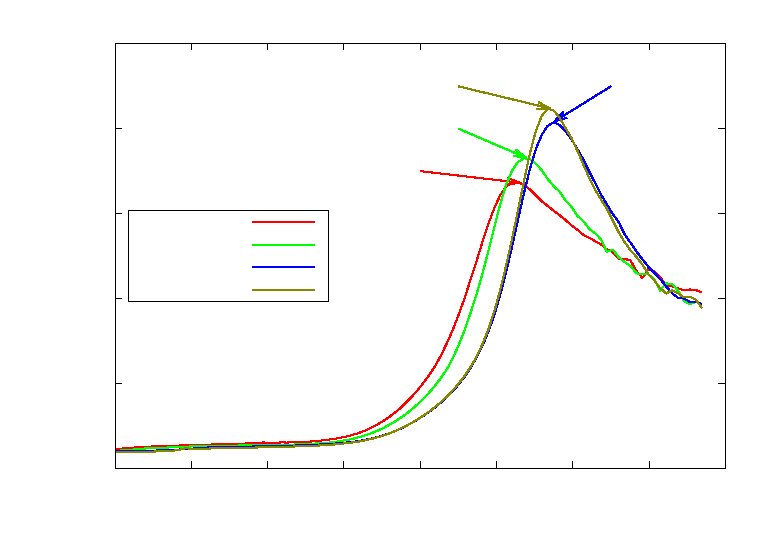
\includegraphics{src/origin/1/tg}}%
    \gplfronttext
  \end{picture}%
\endgroup

    \end{center}
    \caption{外润滑剂玻璃化转变温度}
\end{figure}